%%%%%%%%%%%%%%%%%%%%%%%%%%%%%%%%%%%%%%%%%%%%%%%%%%%%%%%%%%%%%%%%%%%%%%
%%                     Production
%%%%%%%%%%%%%%%%%%%%%%%%%%%%%%%%%%%%%%%%%%%%%%%%%%%%%%%%%%%%%%%%%%%%%%
%\color{blue}
\subsection{Glyph: \glyph{Production}}\label{sec:production}

\glyph{Production} is the arc used to represent the fact that an entity is 
produced by a process. In the case of a reversible transition, the 
\glyph{production} arc also acts as a \glyph{consumption} arc.

\begin{glyphDescription}
 \item[SBO]\mbox{}\\ To be determined.
 \item[origin]\mbox{}\\ Any process node (section~\ref{sec:PNs}), or module (section~\ref{sec:submap}).
 \item[target]\mbox{}\\ Any EPN (section \ref{sec:EPNs}).
 \item[end-points]\mbox{}\\ The target extremity of a \glyph{production} carries a filled arrowhead.
 \end{glyphDescription}

A cardinality label can be associated with \glyph{production} arc indicating the stoichiometry of a process.

\begin{figure}[H]
  \centering
  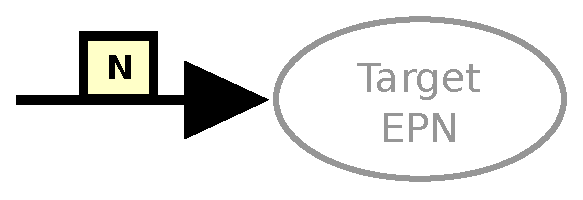
\includegraphics[scale = 0.5]{images/production}
  \caption{The \PD glyph for \glyph{production}.}
  \label{fig:production}
\end{figure}

The following example illustrate the use of consumption/production arc cardinality labels to represent the stoichiometry of a process.

\begin{center}
\scalebox{0.9}{\includegraphics{examples/stoichEx1}}
\end{center}

\normalcolor
